\clearpage
\chapter{Mini Project 3}

\section{Pixel Spreadsheet}
\horizontalline{0}{0}

% Problem 1
\begin{problem}{Problem 1}
    \begin{statement}{Problem Statement}
        Try out the educational app at \href{https://phet.colorado.edu/sims/html/function-builder-basics/latest/function-builder-basics_en.html}{PHet}. What do the functions ?A, ?B, and ?C do to the image cards? Explain each and the process you used to figure it out.
    \end{statement}

    \begin{highlight}[Solution]
        The functions ?A, ?B, ?C all manipulate images in some manner. Some of the images that are in the simulation are symmetric, such as the snowflake and some aren't. Images being symmetric can 
        disguise what these functions do and make it harder to determine what each one is actually doing. I will now explain what each of these functions are doing and how I determined what they do.

        \textbf{?A} is a function that rotates an image $180^{\circ}$. This function essentially flips an image upside down from top to bottom of the image. This is why it is difficult to understand 
        what is happening with the image of the feet and the snowflake. When these images are flipped they look the exact same. When the image of the butterfly and person are flipped it is very evident 
        that the function ?A is flipping an image upside down. This function rotates an image $180^{\circ}$ where the axis of rotation is going in and out of the screen.

        \textbf{?B} is a function that rotates an image clockwise by $90^{\circ}$. I determined that this function was rotating an image clockwise by feeding each individual image through it and seeing 
        what the outcome of the function was producing. For the images that were symmetric, such as the feet and butterfly, it was easy to still see what ?B was doing because it was rotating the images 
        in a plane that was parallel to the screen. This is why the rotation of the snowflake appeared like it wasn't doing anything because the snowflake image is perfectly symmetric. The image that 
        put the nail in the coffin for identifying this rotation was the person because it aligned with the same rotation that was occurring for the feet and butterfly.

        \textbf{?C} is a function that is cutting up each individual image into four sections (like the quadrants in a graph) and positioning them in new locations relative to their original positions. 
        If we use the standard nomenclature for the quadrants in a graph, the block that is originally in quadrant 1 goes to the location of quadrant 4, quadrant 4 goes to quadrant 3, quadrant 3 goes to 
        quadrant 2, and quadrant 2 goes to quadrant 1. This is consistent with each image in the simulation as the results for each image are the same in how they are rearranged. It doesn't matter if 
        they are symmetric or not. This was determined by feeding each image into the function and looking at the output of the image.
    \end{highlight}
\end{problem}

% Problem 2
\begin{problem}{Problem 2}
    \begin{statement}{Problem Statement}
        In the color tutorial we saw that the puppy image was visible even without adding the color formatting to the spreadsheet.

        \begin{enumerate}[label = (\alph*)]
            \item What conditions of this particular image made that possible? Explain.
            \item Do you think all photos will show traces of their image without color information? Explain.
        \end{enumerate}
    \end{statement}

    \begin{highlight}[Solution - Part (a)]
        The image of the puppy is still visible even without adding color formatting to the spreadsheet mainly because of the contrast of pixels that make the outline of the puppy and the contents of 
        the puppy itself. The farther that we zoom out from the image the easier it is to see the contrast of the pixels. The pixels of the puppy itself are lower in value (which correspond to black)
        where as the background behind the puppy are lighter and thus greater in value in comparison to that of the puppy. If it weren't for this stark contrast of the puppy and the background it would
        be a lot more difficult to make out the image of the puppy.
    \end{highlight}

    \begin{highlight}[Solution - Part (b)]
        I don't think that all images show traces of their image because the contrast between the main focus of the image and that of the background can be pretty weak and thus it would make the trace
        of the main object in the image hard to see. The image of the puppy and the background that it is in is very different in color value. The puppy being white, and the background of the puppy being
        green and mix of other colors, generate a stark contrast between the puppy and the background behind it. This is why when we strip the color from the image it is still very easy to make out the
        image of the puppy.

        Take for instance someone's driver license photo. If you wore a shirt that was the same pigment as the background that they use at the DMV, took that image, and then stripped it of its color,
        you probably could only make out the trace of the persons face. This is of course because the contrast of their body and the background that is behind them are similar or the exact same. So I
        don't believe all photos will show traces of their image without color information. This is conveniently a great prank to play while getting your drivers license photo as well!
    \end{highlight}
\end{problem}

% Problem 3
\begin{problem}{Problem 3}
    \begin{statement}{Problem Statement}
        Make a copy of the Puppy Google spreadsheet. Edit this document to give the puppy cool glasses, a hat, or bow tie using a new color recipe from the Swatch spreadsheet. Take a screenshot to 
        document your result. For best results, zoom out. Or download as a PDF, select print, portrait, and fit to width, then screenshot. Insert a screenshot here of the result with a few words about 
        what you did.
    \end{statement}

    \begin{highlight}[Solution]
        \begin{center}
            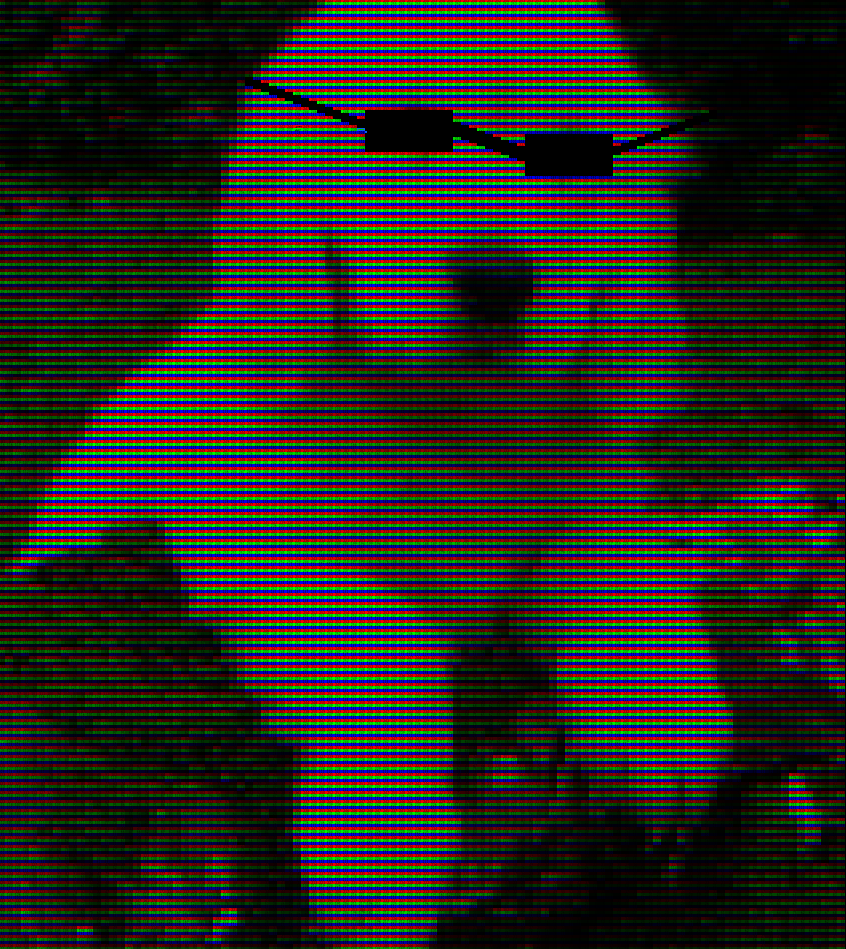
\includegraphics[width = 0.8\textwidth]{Images/Puppy.png}
        \end{center}
        I attempted to add sunglasses to the puppy by going to select pixels in the spreadsheet and making the pixel in question 0. This allowed me to add sunglasses to the puppy. I could of went in and
        finely tuned some of the values to make it look more realistic but I feel like it would still be really pixelated so I just left it the way that it was.
    \end{highlight}
\end{problem}

% Problem 4
\begin{problem}{Problem 4}
    \begin{statement}{Problem Statement}
        Explain what we would need to do to make a negative or inverted image of the puppy. What value would you add or subtract? Explain in detail. Do not do this to the whole image, but try an example 
        on a couple cells and include 2  small screenshots of the before/negative image. (or if you are an Excel master - flip the whole thing and explain your result)
    \end{statement}

    \begin{highlight}[Solution]
        To generate the negative of an image, we need to subtract the current value in red, green, or blue from 255. For each pixel in RGB we need to do the following to calculate the new value
        \begin{align*}
            R* & = 255 - R \\
            G* & = 255 - G \\
            B* & = 255 - B 
        \end{align*}
        where $R*,G*,B*$ all represent the inverted pixels. Take for instance the original snippet of pixels below.

        \begin{center}
            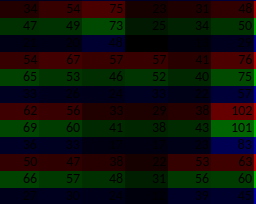
\includegraphics[width=0.25\textwidth]{Images/Original.png}
        \end{center}
        The negative of these pixels can be seen below.

        \begin{center}
            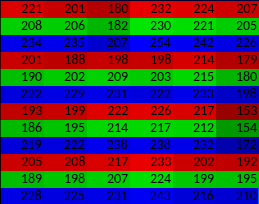
\includegraphics[width=0.25\textwidth]{Images/New.png}
        \end{center}
        Most of this image is either very bright or very dark so the negatives are kind of hard to see up close. But when you zoom out you can see this difference. For instance, if you take the negatives
        of the dogs eyes then it will appear like the dog doesn't even have an eye. Here we just inverted a dark part of the image and now it is bright.
    \end{highlight}
\end{problem}

% Problem 5
\begin{problem}{Problem 5}
    \begin{statement}{Problem Statement}
        Find a photo (Portrait orientation) you have taken (or from the internet) and make a Pixel Spreadsheet from the link on page 9 of the tutorial. The photo should be relatively simple, like the 
        examples, and not have too much detail. Faces work great. If you do not have EXCEL, download the file into Google docs and save as a Google Sheet. Take a screenshot of your Pixel spreadsheet 
        zoomed out enough to see the image and upload here.
    \end{statement}

    \begin{highlight}[Solution]
        I took an image of my favorite football teams logo. Below is the excel spreadsheet after converting it to an image.

        \begin{center}
            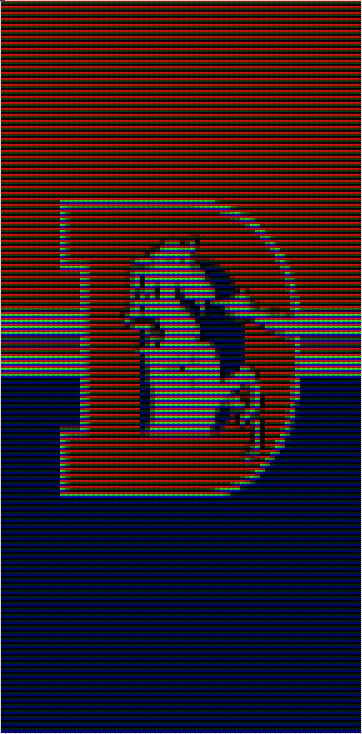
\includegraphics[width=0.5\textwidth]{Images/Broncos.png}
        \end{center}
    \end{highlight}
\end{problem}

% Problem 6
\begin{problem}{Problem 6}
    \begin{statement}{Problem Statement}
        Now use some “hands on Photoshop” to improve the image. Lighten? Darken? Add features? Upload your new photo spreadsheet here and in the space above the photo(s). Explain what “Hands On Photoshop” 
        you did and why. (Since this is the last question you can use as many pages as you need.)
    \end{statement}

    \begin{highlight}[Solution]
        Below is a modified logo of the Broncos head to match the colors of my high school colors.
        \begin{center}
            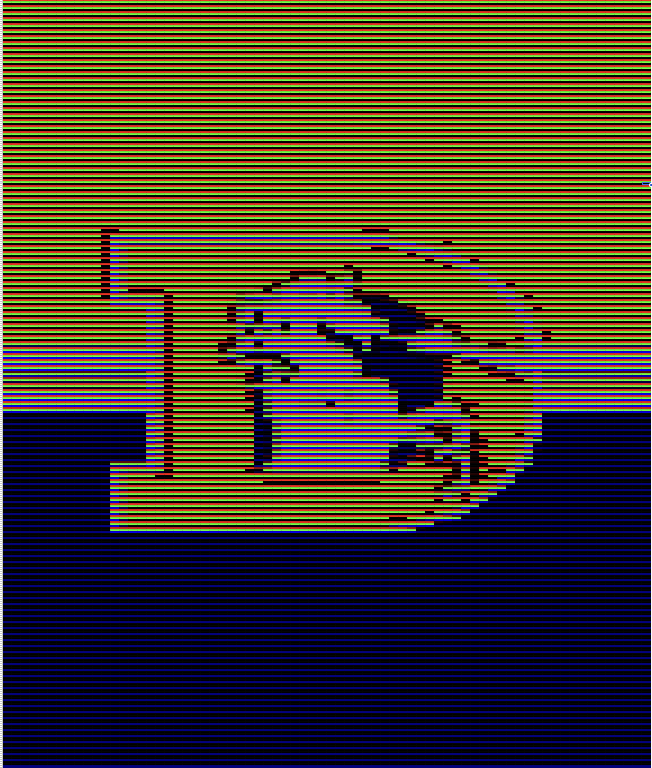
\includegraphics[width=0.7\textwidth]{Images/Broncos Recolored.png}
        \end{center}
        For this change, I wanted to tinker with the oranges in the original image and try to change the scheme of the image as much as I could. I opened up Google sheets and played with values of the 
        orange cells to achieve this new effect. After tinkering with it a lot, I got a more yellow hue of the orange cells and completely changed the color complexion of the original image. I managed to 
        do this by changing the maximum and minimum values in the conditional formatting option inside the spreadsheet. I didn't bother changing the blues as much. My goal was to generate a picture of the
        Broncos image that matched the color complexion of my high school colors, blue and gold.
    \end{highlight}
\end{problem}